 
Firstly it is important to understand how much the way chosen to calculate the power at an output could affect the phases relations and visibilities. This part present the impact of the surface over which is calculated the power on the resulting phases relations and visibilities.

Considering  only 3 distinct wave-guides of the DBC Zig-Zag component. The cross section of each WG is a rectangle $width \times height$. In such a dielectric wave-guide, there is no analytical solution to the scalar wave equation but according to \cite{labeye} a good approximation of the transverse field profile is close to a gaussian :
$$
\Psi(x,y) \approx \Psi_0 exp\left( \frac{-x^2}{\omega_x^2} + \frac{-y^2}{\omega_y^2}\right)
$$

Using this equation and retrieving $\omega_x$ and $\omega_y$ from BeamProp simulation by the width of the gaussian at $1/e$ of its maximal amplitude, we can <<calculate>> the transverse field profile in the wave-guide.

We simulate this behaviour for the following parameters (in $\si{\micro\meter}$) :
\begin{itemize}
    \setlength\itemsep{0pt}
\item[-] Px =24
\item[-] Py = 10.8
\item[-] width = 9.5
\item[-] height = 17
\item[-] $n_{clad}$ = 2.31
\item[-] $\delta n$ = 0.005
\end{itemize}
In this case we have $\omega_x \approx 7.798$ and $\omega_y \approx
10.114$. The resulting field for 3 outputs in phase and guiding the same
power is shown in Fig. \ref{fig:3gauss}.

\begin{figure}[htbp]
  \centering
  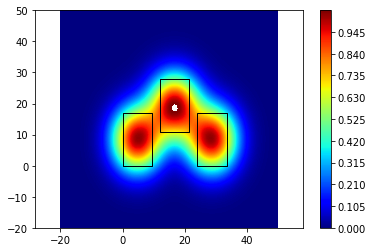
\includegraphics[scale=.5]{picture/integrating_area/3gauss.png}
  \caption{Example of 3 outputs in phase guiding the same power. The modes are Gaussian perfectly centred on the wave-guide}
  \label{fig:3gauss}
\end{figure}

One can see that in this case, where the 3 outputs are in phase, the
determination of the power in the middle WG will be badly estimated by
a simple power integral as : 
\begin{equation} \label{Eq:powerint}
P \propto \iint_{\mathbb{R}^2}
  \Psi^*(x,y)\Psi_{sim}(x,y) dxdy
  \end{equation}
  where $\Psi_{sim}$ is the simulated
output fields as shown on the upper figure. Therefore the integration
should be limited to a user-defined area around the WG. In the next
paragraph we try to have a first feeling of the impact of this choice on the phases
relations, instrumental visibilities and of course the V2PM matrix.

\paragraph{Power of a Gaussian field :}

For an isolated gaussian field the power $P$ is given by \[ \frac{P}{\Psi_0^2} \propto \iint_{\mathbb{R}^2} exp\left( \frac{-2x^2}{\omega_x^2} + \frac{-2y^2}{\omega_y^2} \right) dx dy = \frac{\pi}{2} \omega_x \omega_y\]
In the case of our parameters it is equal to 123.88
$\si{\micro\meter}^2$  (a numerical
integration using the composite trapezoidal rule lead to 123.76). By integrating the whole field as represented
in Fig. \ref{fig:3gauss} we obtain 113.70 $\si{\micro\meter}^2$ but
the truly guided power in the central wave-guide calculated over the
cross-section should only be 87.39 $\si{\micro\meter}^2$ thus an error
of 30 \%. \\
In the opposite case where there is no power in the central
wave-guide, and a maximal power in the two surrounding wave-guides we
find a  guided power in the central wave-guide over the
cross-section of 3.10 $\si{\micro\meter}^2$. It can easily be
understood that the simulated (ergo the experimental) interferograms
will depend of the considered area. The larger this area, the greater
the impact of the surrounding wave-guides on the interferogram.

\paragraph{Influence on the simulated phases relations :}

We have seen that the integrating area used to estimate the guided
power should have a great
impact on the result, we now try to see its impact on the simulated
phase relations. To do this the 3 gaussian are multiplied by a cosine
to simulate a phase dependency. The left and right outputs are set
with phases pi/3 and 2pi/3 respectively and the middle one with phase
0. The power is then integrated on different area centred the WG
cross-section.

One can see that in this case, the phase of the output signal is
mostly unchanged by the integrating area, but this is only the case
for area slightly larger to the WG's cross section. Therefore it
might be expected that the phase relation between outputs with
comparable power magnitude will stay the same for low variation of the
integrating area. The only changed parameter might be the Visibilities
but one can not conclude as the mean value, ergo the photometries changes too.

To this point we have only seen the impact of the integrating area when all outputs are guiding the same maximal power. It is now studied the impact on a low guided power in the middle WG
comparatively to the left and right ones. Same phases are
introduced. The power in the left and right WG are the same and 4
times the power in the middle WG. The results to those simulations are
shown in Fig. \ref{fig:phase_influence}
\begin{figure}[htbp]
  \centering
  \begin{minipage}[b]{.33\textwidth}
    \centering
  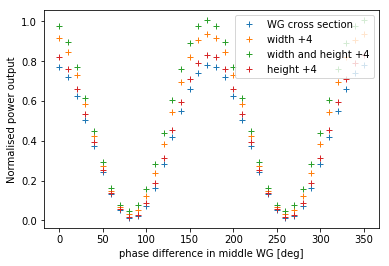
\includegraphics[scale=.35]{picture/integrating_area/phase_python1.png}
    \subcaption{Simulation with the same power in the middle and the surroundings WG.}
  \end{minipage}%
  \hspace{0.2 cm}
  \begin{minipage}[b]{.33\textwidth}
    \centering   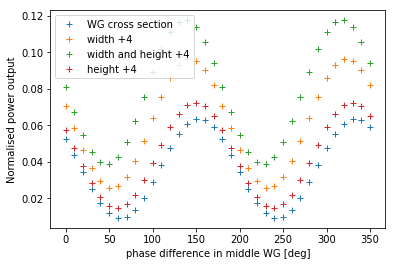
\includegraphics[scale=.35]{picture/integrating_area/phase_python2.png}
    \subcaption{Simulation with low power in the middle WG and high in
    the surroundings.}
  \end{minipage}%
  \hspace{0.2 cm}
  \begin{minipage}[b]{.33\textwidth}
    \centering   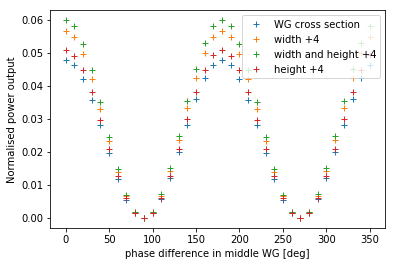
\includegraphics[scale=.35]{picture/integrating_area/phase_python3.png}
    \subcaption{Simulation with low power in the middle WG and high in   \label{fig:forfanout}
    the surroundings for a higher x spacing between the WG.}
  \end{minipage}
  \caption{Influence of different parameters on the phases and
    amplitudes of the interferogram in the middle wave-guide. The phases relations between the outputs are highly influenced by the evanescent coupling}
  \label{fig:phase_influence}
\end{figure}

As can be seen, the more the power difference between the middle WG
and the sides WG and the larger the integrating area, the more
impacted the retrieved phase differences. Therefore it seems that the V2PM matrix of the component should be calculated not only for the isolated component but also with the imaging system. One way to get rid of these dependency would be to have a greater spacing between the WG at the output so that the evanescent coupling is as low as possible (as shown in Fig. \ref{fig:forfanout}). Thus the use of a
<<fan out>> could be an option to have calculate the power over a larger area thus have  a greater integrated power
(ergo a smaller signal to noise ratio (SNR)).
